\documentclass[dvipdfmx]{beamer}
\usepackage{pxjahyper}
%\usetheme{Frankfurt}%Frankfurt,AnnArbor, Antibes, Berlin, Berkeley, Bergen, Boadilla, boxes, Copenhagen

%\beamerdefaultoverlayspecification{<+->}% 箇条書きを段階的にみせたいとき
%\setbeamercovered{transparent}%隠してるアイテムを半透明で表示
\renewcommand{\kanjifamilydefault}{\gtdefault}%日本語フォントをゴシックに
\usepackage{graphicx}% 各種画像の張り込み

%\usepackage[english]{babel}%多言語文書を作成する
\usepackage{amsmath,amssymb}%標準数式表現を拡大する


%----------- ここからスライド内容 ---------------%

%表紙
\title[Slides with Beamer]{ゼミ発表}
%\subtitle{サブタイトル}

\institute{西田研究室}
\author[Hanako Daito]{津上祐典}

\date[June 12 2013]{2016年6月23日}
\subject{\LaTeX{}+Beamer}

%タイトルの表示
\begin{document}
\begin{frame}
 \titlepage 
\end{frame}

%目次の設定
\begin{frame}<beamer> 
  \frametitle{目次}
  \tableofcontents
\end{frame}

\section{はじめに} %目次に表示するスライド名
\begin{frame}{何を問題としているか} %スライドのタイトル
 \begin{itemize}
  \item こんなこと
  \item あんなこと
  \item しかも\alert{そんなことまで}
 \end{itemize}
\end{frame} 

\section{手始めに}

\subsection{Blockの使い方}
\begin{frame}{さまざまなBlock}
\begin{block}{ブロック} 
これがblock環境だ。
\end{block}
\begin{example}
これはexample blockである。
\end{example}

\pause %アニメーション:後から表示する
\begin{alertblock}{警告ブロック}
alert block環境ではこうなる。
\end{alertblock}
\end{frame}



\section{図表の貼り込み}

\subsection{図}

\begin{frame}{PDF画像}
PDF形式の画像も、xbbファイル(extractbbで生成する)を用意しておけば、この通り。
\begin{figure}
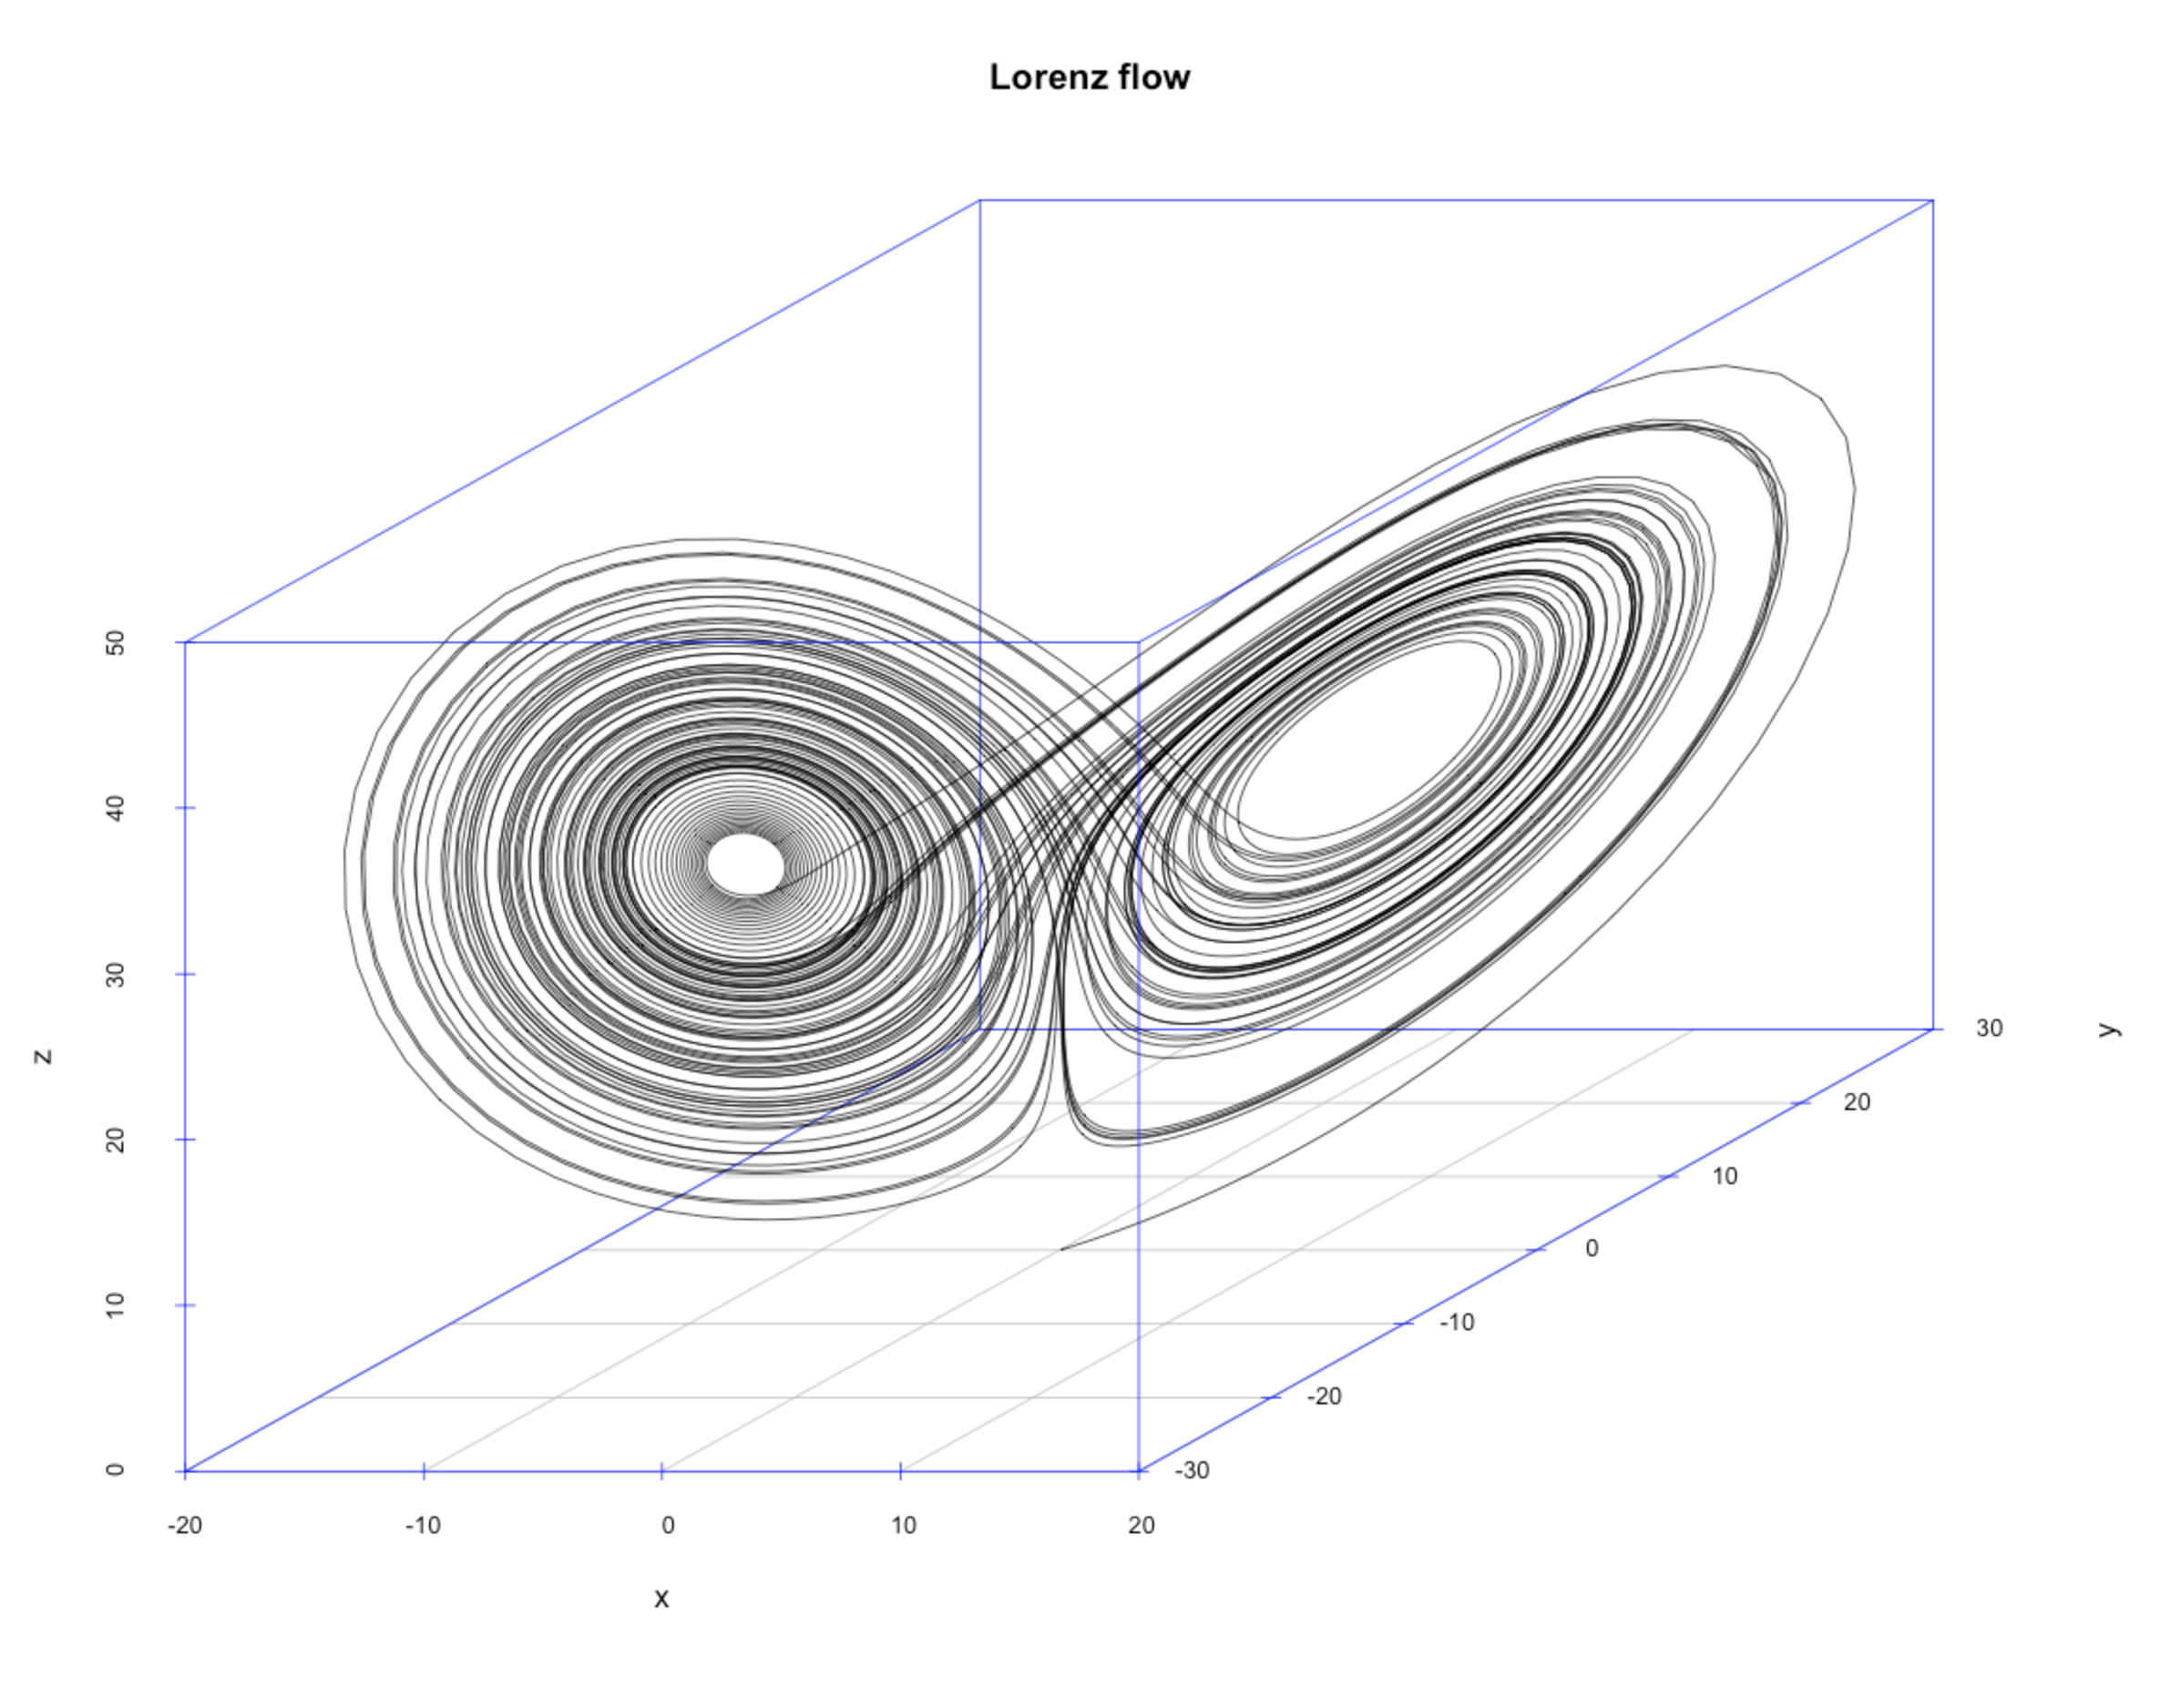
\includegraphics[scale=0.21]{image/lorenz_flow.pdf}
\end{figure}
\end{frame}

\end{document}
